% ----------------------------------------- %
%	Capítulo Exemplo (faça testes aqui)
% ----------------------------------------- %
% ============================================================
% comando para customizar o número das seções (não mexer)
%\renewcommand{\thesection}{\arabic{chapter}.\arabic{section}}
% ============================================================
% Use esse capítulo para testes. Depois comente esse
% arquivo em "principal.tex" para não ser exibido no
% documento final.

\chapter{Capítulo Exemplo}\label{chp:exemplos}

\begin{resumocapitulo}
Esse é apenas um capítulo de demonstração. Inserir alguns comandos em \LaTeX{} para desenvolvimento deste modelo. Não há necessidade de deletar o material que está neste capítulo, apenas vá no arquivo \texttt{principal.tex} e comente ( coloque o símbolo: \%) na linha onde está o nome do arquivo que representa esse capítulo (\texttt{exemplo.tex}).
\end{resumocapitulo}

%-------------------------- %
% Glossário                 %
%-------------------------- %
\section{Como habilitar glossário}

\begin{enumerate}
    \item No preambulo do arquivo {\color{red}$\backslash$\texttt{principal.tex}} (em: \% glossário...) habilitar:
    \begin{enumerate}
        \item IfSubStringInString
        \item usepackage\{glossaries\}
        \item makeglossaries
        \item 31\_glossario
    \end{enumerate}
    \item No corpo do arquivo {\color{red}$\backslash$\texttt{principal.tex}} (procurar no final da página) habilitar:
    \begin{enumerate}
        \item $\backslash$printglossaries
    \end{enumerate}
    \item No arquivo {\color{red}\texttt{31\_glossario.tex}}:
    \begin{enumerate}
        \item Escreva as entradas (expressões) para o glóssario.
        \item siga o exemplo da página ou acesse a \hyperlink{https://pt.overleaf.com/learn/latex/Glossaries}{página no Overleaf} para maiores detalhes.
        \item {\color{red}Atenção:} coloque primeiro a expressão no Glossário (arquivo: 31\_glossario.tex) antes de usar no texto principal.
    \end{enumerate}
\end{enumerate}

\subsection{Exemplo de como usar termos do Glossário}

%The \texttt{glossaries} package automatically generates a list of glossary entries. It's great for keeping track of your \gls{domain-knowledge} and \glspl{tla}. In this example we've put the glossary definitions in a separate \texttt{glossary.tex} file, which you can edit via the project menu.

%---------------------------------------------------------------
\newpage
%-------------------------- %
% Notas de rodapé           %
%-------------------------- %
\section{Notas de rodapé}
Esse documento foi desenvolvido com base no modelo do PPGI-UNINOVE\footnote{Universidade Nove de Julho}, de autoria de Charles Ferreira Gobber.
É uma extensão do template do IME-USP\footnote{Instituto de Matemática e Estatística} desenvolvido pelo professor Jesús P. Mena-Chalco.

\textit{Para saber mais sobre nota de rodapé acesse \hyperlink{https://pt.overleaf.com/learn/latex/Footnotes}{Overleaf}}.
%-------------------------- %
% Hierárquia de seções      %
%-------------------------- %
\section{Hierarquia de seções}
\begin{itemize}
    \item $\backslash$chapter{}
    \begin{itemize}
        \item $\backslash$section{}
        \begin{itemize}
            \item $\backslash$subsection{}
            \begin{itemize}
                \item $\backslash$subsubsection{}
            \end{itemize}
        \end{itemize}
    \end{itemize}
\end{itemize}

%---------------------------------------------------------------
\newpage
%-------------------------- %
% Figuras                   %
%-------------------------- %
\section{Exemplo de figuras}
Consideram-se figuras os desenhos, mapas, esquemas, gráficos, fórmulas, modelos, fotografias, diagramas, fluxogramas, organogramas, entre outros.

Pelas normas da ABNT as figuras devem ser adicionadas com um título em cima e a fonte em baixo. Depois deve ser referenciada no texto o mais próximo possível. \textbf{Todas figuras inseridas devem ser referenciadas}, por exemplo (Figura~\ref{fig:estr_trab_academicos}).
Neste documento, organize as figuras na pasta \texttt{figuras}.
% Figura 1 ............................................................

\begin{figure}[htbp]
\hypertarget{arquitetura}{%
\caption{Estrutura de Trabalhos Acadêmicos}\label{fig:estr_trab_academicos}
\begin{center}
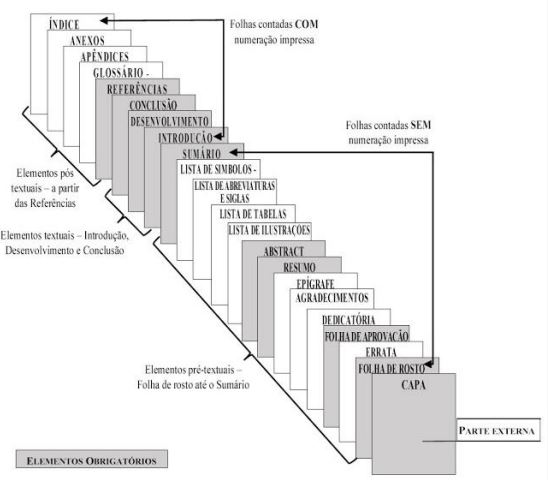
\includegraphics{material-de-apoio/figuras/estrutura_monografias.JPG}\\
\fonte{Manual de Trabalhos Acadêmicos UNINOVE}
\end{center}
}
\end{figure}

Maiores detalhes de como customizar figuras, inserir figuras no meio do texto, rotacionar etc consultar os materiais:
\begin{itemize}
    \item \hyperlink{https://www.ime.unicamp.br/~marchesi/Allegati/NotasdeAulaLaTeX.pdf}{IMEC-UNICAMP Notas de Aula \LaTeX{}}, página 26.
    \item \hyperlink{http://www.uel.br/projetos/matessencial/superior/pdfs/latexmat.pdf}{\LaTeX{} para Matemática - Departamento de Matemática UEL}, página 60.
\end{itemize}
%---------------------------------------------------------------
\newpage
%-------------------------- %
% Equações                  %
%-------------------------- %
\section{Exemplo de expressões matemáticas}

% Equação exemplo .........................................................
% Exemplo de equação
\begin{equation}\label{eq:Eq1}
   a=b
\end{equation}
\myequations{Equation number \ref{eq:Eq1}}


Equação~\ref{eq:Eq1}

%-----------------------------
\begin{itemize}
    \item \textbf{Sites interessantes para expressões e símbolos matemáticos:}
    \begin{itemize}
        \item \hyperlink{https://pt.overleaf.com/learn/latex/Mathematical_expressions}{Mathematical expressions - Overleaf.}
        \item \hyperlink{http://tug.ctan.org/info/short-math-guide/short-math-guide.pdf}{Short Math Guide for \LaTeX{}}
        \item \hyperlink{http://www.ams.org/arc/tex/amsmath/amsldoc.pdf}{User's Guide for the \texttt{amsmath} Package}
        \item \hyperlink{https://www.ime.unicamp.br/~marchesi/Allegati/NotasdeAulaLaTeX.pdf}{IMEC-UNICAMP Notas de Aula \LaTeX{}}
    \end{itemize}
\end{itemize}

%---------------------------------------------------------------
\newpage
%-------------------------- %
% Quadros e tabelas         %
%-------------------------- %
% Exemplo de quadro ..............................................
\section{Exemplo de quadro e tabela}
Quadros são formados por linhas verticais e horizontais, deem ter todas extremidades fechadas e, geralmente, são utilizados para \textbf{dados qualitativos}.

A diferença do quadro pra tabela é que o quadro tem linhas verticais.
Quadro~\ref{quad:exemplo_de_quadro}

% Exemplo de quadro

\begin{quadro}[!ht]
%\caption{Quadro de Exemplo}\label{quad:exemplo_de_quadro}
\caption{\label{quad:exemplo_de_quadro}Quadro de Exemplo}
\centering
\begin{tabular}{ |p{3cm}||p{3cm}|p{3cm}|p{3cm}|  }
\hline
\multicolumn{4}{|c|}{Country List} \\
\hline
Country & ISO ALPHA 2 & ISO ALPHA 3 & ISO Code\\
\hline
Afghanistan   & AF    &AFG&   004\\
Aland Islands&   AX  & ALA   &248\\
Albania &AL & ALB&  008\\
Algeria    &DZ & DZA&  012\\
American Samoa&   AS  & ASM&016\\
Andorra& AD  & AND   &020\\
Angola& AO  & AGO&024\\
\hline
\end{tabular}
\vskip 0.2cm
\fonte{Adaptado de \hyperlink{https://pt.overleaf.com/learn/latex/Tables}{Overleaf}}
\end{quadro}
\vspace{0em}
\footnotesize Se usar o comando \texttt{fonte} dentro do ambiente da tabela a "fonte" fica centralizada, caso contrário fica fora.

\begin{itemize}
    \item Para maiores detalhes de como fazer quadros veja:
    \begin{itemize}
        \item \hyperlink{https://wp.ufpel.edu.br/diehl/files/2017/06/aula11_ccf.pdf}{Comunicação Científica em Física}.
    \end{itemize}
\end{itemize}

\hrulefill

% Exemplo de tabela ..............................................
Enquanto os quadros são fechados e apresentam dados qualitativos,
as tabelas são abertas e apresentam dados estatísticos numéricos.
Linhas horizontais só se admitem no cabeçalho e no rodapé.
\begin{itemize}
    \item \textbf{Não deve figurar dados em branco:}
    \begin{itemize}
        \item Traço indica dado inexistente
        \item Reticências indicam dado desconhecido
        \item Zero deve ser usado quando o dado for menor que a metade da unidade adotada para a expressão do dado
    \end{itemize}
\end{itemize}

A ilustração a seguir (Tabela~\ref{quad:exemplo_de_quadro}) é um exemplo de quadro, pelas normas da ABNT.
% Exemplo de tabela
% Fonte: http://www1.maths.leeds.ac.uk/LaTeX/TableHelp1.pdf
\begin{table}[h]
\label{tab:exemplo}
\caption{Tabela de Exemplo} % title name of the table
\centering % centering table
\begin{tabular}{l c c rrrrrrr} % creating 10 columns
\hline\hline % inserting double-line
 Audio &Audibility & Decision &\multicolumn{7}{c}{Sum of Extracted Bits}
\\ [0.5ex]
\hline % inserts single-line
% Entering 1st row
 & &soft &1 & $-1$ & 1 & 1 & $-1$ & $-1$ & 1 \\[-1ex]
\raisebox{1.5ex}{Police} & \raisebox{1.5ex}{5}&hard
& 2 & $-4$ & 4 & 4 & $-2$ & $-4$ & 4 \\[1ex]
% Entering 2nd row
& &soft & 1 & $-1$ & 1 & 1 & $-1$ & $-1$ & 1 \\[-1ex]
\raisebox{1.5ex}{Beethoven} & \raisebox{1.5ex}{5}& hard
&8 & $-8$ & 2 & 8 & $-8$ & $-8$ & 6 \\[1ex]
% Entering 3rd row
& &soft & 1 & $-1$ & 1 & 1 & $-1$ & $-1$ & 1 \\[-1ex]
\raisebox{1.5ex}{Metallica} & \raisebox{1.5ex}{5}& hard
&4 & $-8$ & 8 & 4 & $-8$ & $-8$ & 8 \\[1ex]
% [1ex] adds vertical space
\hline % inserts single-line
\end{tabular}
\vskip 0.2cm
\fonte{Adaptado de \hyperlink{http://www1.maths.leeds.ac.uk/LaTeX/TableHelp1.pdf}{Creating Tables with \LaTeX{}}}
\end{table}

%---------------------------------------------------------------
\newpage
%-------------------------- %
% Mapas                     %
%-------------------------- %
\section{Exemplo de mapas}
Inserir o mais próximo do texto a que se referem.
No topo da imagem inserir o título.
Centralizar imagem, título, legenda e fonte.
Utilizar fonte 10.
Na parte inferior citar a fonte (mesmo que seja o próprio autor).

O Mapa~\ref{map:brasil_mapa} representa as UFs do Brasil.

\begin{mapa}[H]
\centering
\caption{Mapa do Brasil}\label{map:brasil_mapa}
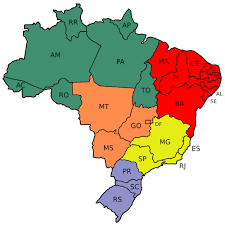
\includegraphics[scale=0.9]{material-de-apoio/mapas/mapa-do-brasil.png}\\
\fonte{Google}
\end{mapa}

%---------------------------------------------------------------
\newpage
%-------------------------- %
% Algoritmos                %
%-------------------------- %

Exemplo de pseudocódigo utilizando o pacote {\color{red}algorithm2e}:

% Exemplo de algoritmo:
% controla endentação
\begin{algorithm}[H]
\SetAlgoLined
\Entrada{$S,\eta, U$} 
\Saida{Número esperado de nós atingidos}
\Inicio{
	$\sigma(S) = 0$ \\
\Para{cada $u \in S$}{
	$\sigma(S)\leftarrow \sigma(S)+\textsc{Backtrack}(u,\eta,W,U)$\\
}
}
\Retorna{$\sigma(S)$}
\label{alg1}
\caption{\textsc{Esperança}}
\end{algorithm}

%---------------------------------------------------------------
\newpage
%-------------------------- %
% Índice Remissivo          %
%-------------------------- %
\section{Exemplo de Índice Remissivo}
Para criar um índice remissivo devemos usar o pacote \texttt{makeidx} e dar o comando
\texttt{$backslash$makeindex} no preâmbulo do documento para inicializá-lo.

Cada entrada do índice é adicionada logo após a ocorrência da mesma da seguinte forma:

$backslach$\{chave\}, onde a \textit{chave} é o texto que aparecerá no índice (com a página correspondente). Se uma mesma chave aparecer mais de uma vez no texto ela aparecerá uma única vez no índice, com os números das páginas das ocorrências. É possível incluir suentradas e s subsubentradas de uma entrada colocando "\!" entre elas.

Para maiores detalhes acesse o documento online: \hyperlink{https://www.ime.usp.br/~viviane/MAP2212/minicurso.pdf}{Minicurso de \LaTeX{}}.
Ou \hyperlink{https://netsgo.wordpress.com/2010/09/28/aprenda-a-criar-um-indice-remissivo-no-latex-learning-how-to-create-an-index-with-latex/}{Aprenda a criar um índice remissivo no \LaTeX{}}.

Exemplo:
\begin{itemize}
    \item \index{Amplificador ótico} é um equipamento responsável por amplificar o sinal óptico proveniente do transmissor de vídeo.
    \item \index{Amplificaro ótico!EDFA} do inglês \textit{Erbium Doped Fiber Amplifier}.
\end{itemize}